\chapter{Mathematical Background}
\label{ch:app:mathtools}

We collect here some basic useful facts, all of which can be found in 
standard textbooks 
on calculus and discrete mathematics, to which the reader should refer for proofs.

\section{Sets}
\label{sec:app:sets}

A \defnfont{set} is a collection of distinguishable objects  
(its \defnfont{elements}) whose order is 
unimportant. Two sets are the same if and only if they have the same elements.
We denote the statement that $x$ is an element of the set $X$ by $x\in X$ and the 
negation of this statement by $x\not\in X$.
We can list finite sets using the braces notation: for example, the set $S$ 
consisting 
of all integers between 1 and 10 that are divisible by 3 is denoted $\{3, 6, 9\}$. 
A \defnfont{subset} of a set $X$ is a set all of whose elements are also elements of 
$X$. Each set has precisely one subset with zero elements, the \defnfont{empty set} 
which is denoted $\emptyset$. A subset can be described by 
set-builder notation; 
for example, the subset of $S$ consisting of 
all multiples of $3$ between $1$ and $7$ can be written
$\{s \mid s \in S \text { and } s \leq 7\}$.

For sets $X$ and $Y$, the \defnfont{union} and \defnfont{intersection} 
of $X$ and $Y$ are, respectively, the sets defined as follows
(note that the ``or" is inclusive, so ``$P$ or $Q$" is true if and only if $P$ is true, $Q$ is true, or both $P$ and $Q$ are true):
\begin{align*}
X \cup Y&= \{x \mid x \in X \text{ or } x \in Y\}\\
X \cap Y&=\{x \mid x \in X \text{ and } x \in Y\}.
\end{align*}
The \defnfont{set difference} $X\setminus Y$ is defined by 
$X\setminus Y = \{x \mid x\in X \text{ and } x\not\in Y\}$.
The \defnfont{complement} of a subset $S$ of $X$ is the subset 
$\overline{S} = X\setminus S$ of $S$.  The number of elements
(often called its \defnfont{cardinality}) of
a set $X$ is often denoted by $|X|$.

\section{Mathematical induction}
\label{sec:app:ind}

A common way of proving that a statement $P(n)$ is true for all
integers $n$ after some threshold $n_0$ is as follows. It is called the
\defnfont{principle of mathematical induction} and is equivalent to the
fact that there are no infinite chains of nonnegative integers $x_1 >
x_2 > \dots$.

The principle of mathematical induction states that \boldfont{if} 
\begin{itemize}
\item
$P(n_0)$ is true \boldfont{and}
\item \boldfont{for each} $n\geq n_0$, \boldfont{if} $P(n)$ is true 
\boldfont{then}  $P(n+1)$ is true
\end{itemize}
\boldfont{then} $P(n)$ is true for all $n\geq n_0$.

For example, suppose we wish to prove that there exists some constant
$c>0$ such that $(n+1)^4/n^4 \leq c$ for all $n\geq 1$ (see below for
motivation). We notice that when $n=1$ the ratio is $16$ and that it
appears to get smaller with increasing $n$ (the next few values of the
ratio are $81/16\cong 5$ and $256/81 \cong 3$). So we may guess
that $c=16$ will work (or any larger number). So we have that $n_0 =
1$, $P(n)$ is the statement ``$(n+1)^4/n^4 \leq 16$ for all $n\geq 1$".

We already know that $P(n_0)$ is true. Now suppose that $P(n)$ is true
for some $n\geq n_0$. We need to show that $P(n+1)$ is true. We know that
$$(n+1)^4 \leq 16 n^4$$ and wish to show that $$(n+2)^4 \leq 16 (n+1)^4.$$

Taking 4th roots we have $n+1 \leq 2 n$ and we want $n+2 \leq 2
(n+1)$. Now using the fact that $P(n)$ is true (this is called the
\defnfont{inductive hypothesis}), we have $n+2 = n+1 + 1 \leq 2n + 1 <
2 (n+1)$ so the result follows. Thus $P(n)$ is true for all $n$ by the
principle of mathematical induction.


An alternative form of the principle of mathematical induction, which
is equivalent to it, is called \defnfont{complete induction}:

\begin{itemize}
\item
$P(n_0)$ is true \boldfont{and}
\item \boldfont{for each} $n\geq n_0$, \boldfont{if} $P(i)$ is true for each $i$ 
with $n_0 \leq i \leq n$, \boldfont{then}  $P(n+1)$ is true
\end{itemize}
\boldfont{then} $P(n)$ is true for all $n\geq n_0$.


\section{Relations}
\label{sec:app:relations}

A \defnfont{relation} on a set $S$ is a set $R$ of ordered pairs of
elements of $S$, that is, a subset of $S\times S$. If $(x, y)$ is a such
a pair, we say that $x$ is related to $y$ and sometimes write $x\,R\,y$. An
example is the relation of divisibility on the positive integers;
$x\,R\,y$
if and only if $y$ is a multiple of $x$. Here $2 \,R \, 12$, $1\, R\,
x$ for every $x$, and $x\,R\,1$ only if $x=1$.

There are some special types of relations that are important for our purposes.

An \defnfont{equivalence relation} is a relation that is
\defnfont{reflexive, symmetric} and \defnfont{transitive}. That is,
we have for every $x, y, z\in S$
\begin{itemize}
\item $x R x$

\item if $x R y$ then $y R x$

\item if $x R y$ and $y R z$ then $x R z$

\end{itemize}

An equivalence relation amounts to the same thing as a
\defnfont{partition}: a decomposition of $S$ as a union of disjoint
subsets. Each subset consists of all elements that are related to any
one of them, and no elements in different subsets of the partition
are related.

Examples of equivalence relations: ``having the same mother" on the set of
all humans; ``being divisible by 7" on the set of all positive integers;
``being mutually reachable via a path in a given graph".

Another important type of relation is a \defnfont{partial order}. This
is a relation that is reflexive, \defnfont{antisymmetric} and
transitive. Antisymmetry means that if $x\, R\, y$ and $y\, R\, x$ then
$x=y$. Examples are: $x\, R\, y$ if and only if $x$ is a factor of $y$ ,
where $x$ and $y$ are positive integers.

A \defnfont{linear order} or \defnfont{total order} is a partial order
where every pair of elements is related. For example, the usual relation
$\leq $ on the real numbers. The elements of a finite set with a total
order can be arranged in a line so that each is related to the next and
none is related to any preceding element.

\section{Basic rules of logarithms}

For $x>1, y > 0$, the logarithm \(\log_x y\) to base \(x\) of \(y\) satisfies the equality:
\(
x^{\log_x y} = y
\)
and has the following properties:
\begin{itemize}
\item \(\log_x ( a \cdot b ) = \log_x a + \log_x b\)
\item \(\log_x ( a / b )     = \log_x a - \log_x b\)
\item \(\log_x ( a^b )       = b \log_x a\)
\end{itemize}

Using the definition and the properties of the logarithm,
it is easy to show that the following rules hold for $x>1, y>0, z>0$.
\[
\begin{array}{lll} 
\log_x y & = & \frac{1}{\log_y x}\\
\log_x z & = & \frac{\log_y z}{\log_y x}\\
z^{\log_x y} & = & y^{\log_x z}
\end{array}
\]
The last rule is easily proven by taking logarithm to base
\(x\) of each side of the equality.\\

The notation $\log_{e} = \ln$ is commonly used, as also is $\log_2 = \lg$.

Often we want to convert the real values returned from functions like 
logarithms to integers. Let $x$ be a real number.
The \defnfont{floor} $\lfloor x \rfloor$ of $x$ is the greatest integer 
not greater than $x$, and the \defnfont{ceiling}
$\lceil x \rceil$ of $x$ is the least integer not less than $x$. If $x$ is an integer, then $\lfloor x \rfloor = x = \lceil x \rceil$.

\section{L'H\^{o}pital's rule}
\label{sec:app:lhopital}

This rule was in fact proved by J.~Bernoulli and sold to G.~de~L'H\^{o}pital for 
inclusion in the first calculus textbook, published in 1696. The form that we 
need for asymptotics is as follows.

\begin{Theorem}
If $\lim_{x\to \infty} f(x) = \infty = \lim_{x\to
\infty} g(x)$ and $f, g$ are positive differentiable functions for $x>0$,
then $$\lim_{x\to\infty} f(x)/g(x) = \lim_{x\to\infty} f'(x)/g'(x).$$
\end{Theorem}

As an example, to compute the limit of $e^x/x^3$ as $x\to \infty$, we use 
the rule repeatedly:
$$
\lim_{x\to\infty} \frac{e^x}{x^3} = \lim_{x\to\infty} \frac{e^x}{3x^2} = 
\lim_{x\to\infty} \frac{e^x}{6x} = \lim_{x\to\infty} \frac{e^x}{6} = \infty.
$$

\section{Arithmetic, geometric, and other series}
\label{sec:app:sum:series}

A general arithmetic series is specified by the recurrence
\(a_n = a_{n-1} + c\), where \(c\) is a constant. The sum of
its \(n\) terms is
\[
a_{1}+a_{2}+\ldots+a_{n} = \frac{n}{2}(a_1 + a_n ) =
na_1 + c\frac{n(n-1)}{2}.
\] 
When \(a_1=1\) and \(c=1\), 
\[
1 + 2 + \dots + n = \frac{n(n+1)}{2}
\]

A general geometric series is specified by the recurrence
\(a_n = ca_{n-1}\), where \(c \ne 1\) is a constant. The
sum of its \(n\) terms is
\[
a_{1}+a_{2}+\ldots+a_{n} = a_1 \frac{c^n - 1}{c - 1}
\]
If \(0 < c < 1\), it is better to rewrite the sum as
\[
a_{1}+a_{2}+\ldots+a_{n} = a_1 \frac{1 - c^n}{1-c}
\]
When \(n\) goes to infinity, the sum of the latter
infinite geometric series is
\[
\sum\limits_{k=1}^{\infty}a_k = \frac{a_1}{1-c}
\]
provided $|c| < 1$, otherwise the infinite sum does not exist.

The sum of squares has an easily guessed explicit formula
\[
\sum_{i=1}^n i^2 = 1 + 2^2 + 3^2 + \ldots + n^2 = \frac{n(n+1)(2n+1)}{6}
\]
which can be proved by induction.
Similar explicit formulae hold for the sum $\sum_{i=1}^n i^p$ where $p$
is a fixed positive integer, but they become rather complicated. More
useful for our purposes is the asymptotic formula for large $n$
\[
\sum_{i=1}^n i^p \in \Theta(n^{p+1})
\]
which also holds for negative integers $p$ 
provided $p\neq -1$. When $p= -1 $ we have an asymptotic statement about 
the \defnfont{harmonic numbers} $H_n = \sum_{i=1}^n i^{-1}$,
\[
\sum_{i=1}^n 1/i  \in \Theta(\log n).
\] 

A similar sum of interest to us is $$\log(n!) = \sum_{i=1}^n \log
i.$$ This is in $\Theta(n\log n)$ for any base of the logarithm.

%A explicit related formula is
%\[
%\sum\limits_{k=1}^{n} \lfloor \log_2 k \rfloor =
%(n+1)\lfloor \log_2 n \rfloor - 2^{\lfloor \log_2 n \rfloor + 1} + 2.
%\]

A more complicated formula (\defnfont{Stirling's approximation}),
which we do not prove here, is
$$n! > n^n e^{-n} \sqrt{2 \pi n}$$
and in fact, as $n\to \infty$, we have
$$ n! \approx n^n e^{-n} \sqrt{2 \pi n},$$ 
where $f \approx g$ is a stronger result than $f\in \Theta(g)$, namely 
$\lim_{n\to \infty} f(n)/g(n) = 1$.

The above asymptotic results can all be proved in the following way
using integral calculus. The method works for any continuous function
that is increasing or decreasing (a monotone function) for $x>0$. For
example, consider $f(x) = x^3$ which is increasing. Then we may
approximate the integral $\int_0^n f(x) \, dx$ from below by the sum of
rectangles with base length $1$ and height $f(i)$, the sum going from $0$ to
$n-1$. See Figure~\ref{fig:intapprox}. Similarly we can approximate it
from above by the same sum from $1$ to $n$. This gives after
rearrangement:
$$
\int_1^{n} x^3 \, dx \leq \sum_{i=1}^n i^3 \leq \int_{1}^{n+1} x^3 \, dx
$$
and so we have 
$$\frac{n^4 -1}{4} \leq \sum_{i=1}^n i^3 \leq \frac{(n+1)^4 - 1}{4}.$$
This easily yields that $\sum_{i=1}^n i^3$ is $\Theta(n^4)$ since
$(n+1)^4/n^4 \leq 16$ for $n\geq 1$ and $n^4 - 1 \geq 15n^4/16$ for $n\geq 2$.

\begin{figure}
%\centerline{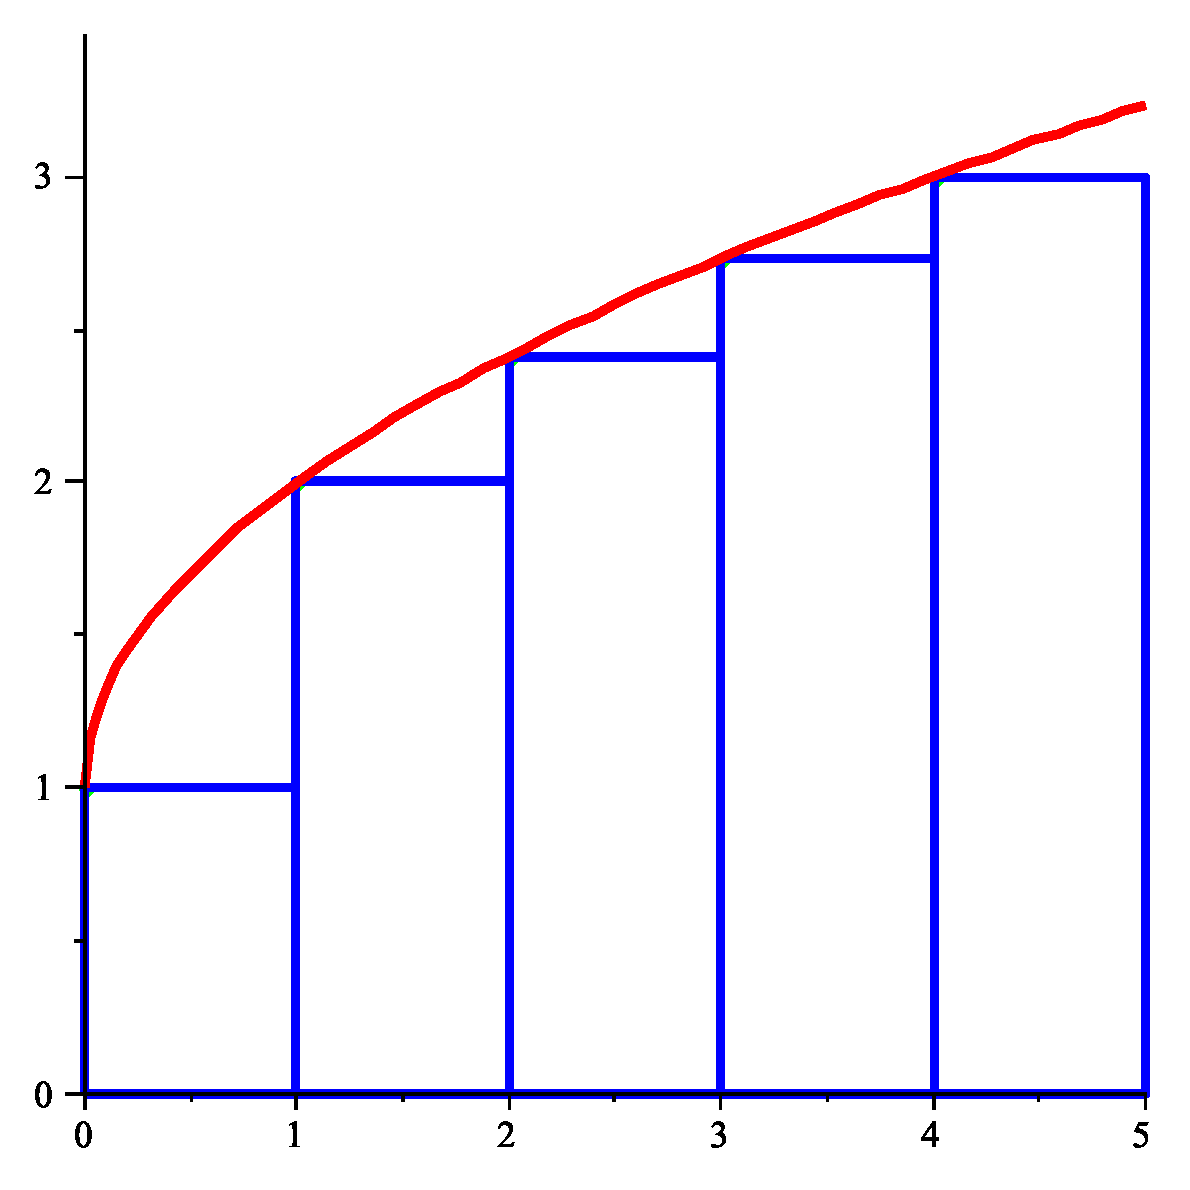
\includegraphics[width=2.3in]{figs/riemann-lower.eps}}
\centerline{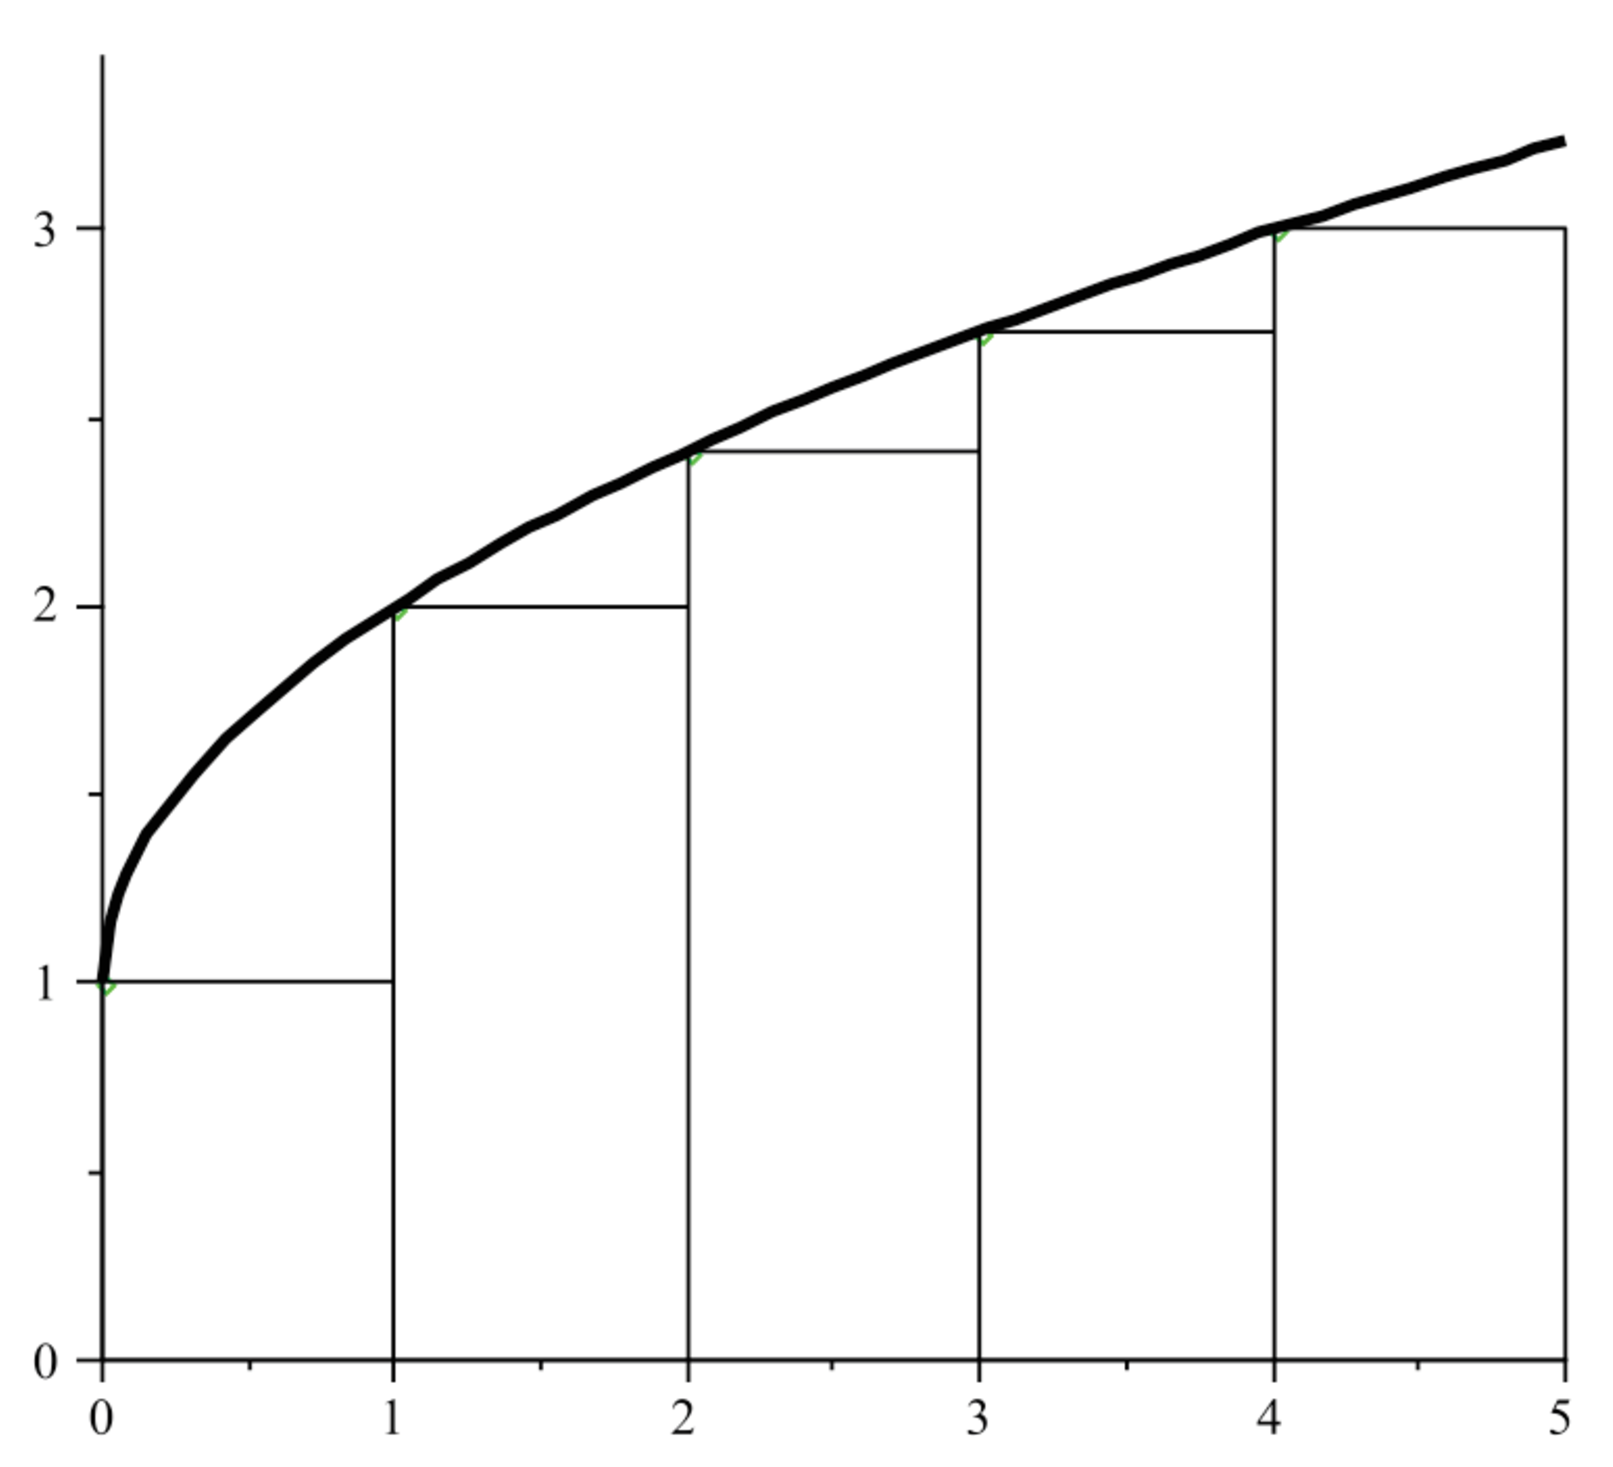
\includegraphics[width=2.3in]{figs/riemann-lower-bw.eps}}
\caption{Approximation of an integral by lower rectangles.}
\label{fig:intapprox}
\end{figure}

\section{Trees}
\label{sec:app:trees}

A \defnfont{rooted ordered tree} is what computer scientists call simply
a ``tree". These trees are defined recursively. An ordered rooted tree
is either a single node or a distinguished node (the \defnfont{root}) 
attached to some ordered rooted trees given in a fixed order 
(hence such a tree is defined recursively). In a picture, these subtrees 
are usually drawn from left to right below the parent node.  
The \defnfont{parent} of a node is defined as follows. The root has no parent. 
Otherwise the node was attached in some recursive call, and the root 
it was attached to at that time is its parent. The roots of the subtrees 
in the definition are the \defnfont{children} of the root. A rooted 
ordered tree can be thought of as a digraph in which there is
an arc from each node to each of its children.

A node with no children is called a \defnfont{leaf}. The \defnfont{depth} of a node
is the distance from the root  to that node (the length of the unique path between 
them). The \defnfont{height of a node} is the length of a longest path from the 
node to a leaf. The \defnfont{height} of tree is the height of the root. Note that
a tree with a single node has height zero. Some other books use a definition of 
height whose value equals the value given by our definition, plus one.

A \defnfont{binary tree} is an ordered rooted tree where the number 
of children of each node is always $0, 1$, or $2$. 

A \defnfont{free tree} (what mathematicians call a tree) has no order 
(so a mirror image of a picture of a tree is a picture of the same tree) 
and no distinguished root. Every free tree can be given a root arbitrarily 
(in $n$ ways, if the number of nodes is $n$), and ordered in many 
different ways. 

A free tree can be thought of as the underlying graph of an 
ordered rooted tree. A free tree is a very special type of graph. First, if $n$ is the number
of nodes and $e$ the number of edges, then $e=n-1$. To see this, note that
in the underlying graph of an ordered rooted tree, each edge connects
a node with its parent. Each node except one has a parent. Thus there
is a one-to-one correspondence between nodes other than the root 
and edges, yielding the result.

\if 11
One can easily show that the following are equivalent for a graph $G$:
\begin{itemize}
\item $G$ is a free tree.
\item $G$ is a connected graph with $e=n-1$.
\item $G$ is an acyclic graph with $e=n-1$.
\end{itemize}
\else
We claim now that a graph is a free tree if and only if it is connected
and has no cycles. First note that a free tree is certainly connected.
Given a connected graph with a cycle, we can delete an edge from the
cycle and still have a connected graph. Thus a connected graph such that
deleting any edge (a minimal connected graph) makes it disconnected
must be acyclic. On the other hand, if we have an acyclic graph such
that adding any edge creates a cycle (a maximal acyclic graph) then it
must be connected (otherwise we could add an edge between two connected
components). So maximal acyclic graphs are the same as minimal connected
ones, and the same as connected acyclic graphs. We claim that they are
the same as free trees.

We prove by induction on $n$ that a connected acyclic graph has
$e=n-1$. It is certainly true if $n=1$. Now note that a connected acyclic
graph must have a vertex of degree $1$. One way to see this to consider
a longest possible path in the graph: the endpoints must have degree
$1$ or else it could be extended. If we delete this degree $1$ vertex,
the resulting graph is still connected and acyclic, so by the inductive
hypothesis, this graph with $e-1$ edges and $n-1$ vertices satisfies
$e-1=n-2$, as required.

Thus a connected graph with a cycle must have $e\geq n$ because we can
delete an edge and maiintain connectedness. Hence every free tree is a
connected acyclic graph.

Similarly, every connected acyclic graph can be considered as a free
tree. For example, we may again use induction. Deleting a degree 1
node $v$ we obtain the underlying graph of some ordered rooted tree,
by induction, and the edge to $v$ can be oriented so $v$ becomes a leaf
in a bigger ordered rooted tree.

Note that we have proved above that a free tree could also be defined
as a connected graph with $e=n-1$ or an acyclic graph with $e=n-1$.
\fi

